\documentclass[twoside]{book}

% Packages required by doxygen
\usepackage{fixltx2e}
\usepackage{calc}
\usepackage{doxygen}
\usepackage[export]{adjustbox} % also loads graphicx
\usepackage{graphicx}
\usepackage[utf8]{inputenc}
\usepackage{makeidx}
\usepackage{multicol}
\usepackage{multirow}
\PassOptionsToPackage{warn}{textcomp}
\usepackage{textcomp}
\usepackage[nointegrals]{wasysym}
\usepackage[table]{xcolor}

% NLS support packages
\usepackage[french]{babel}
\NoAutoSpaceBeforeFDP

% Font selection
\usepackage[T1]{fontenc}
\usepackage[scaled=.90]{helvet}
\usepackage{courier}
\usepackage{amssymb}
\usepackage{sectsty}
\renewcommand{\familydefault}{\sfdefault}
\allsectionsfont{%
  \fontseries{bc}\selectfont%
  \color{darkgray}%
}
\renewcommand{\DoxyLabelFont}{%
  \fontseries{bc}\selectfont%
  \color{darkgray}%
}
\newcommand{\+}{\discretionary{\mbox{\scriptsize$\hookleftarrow$}}{}{}}

% Page & text layout
\usepackage{geometry}
\geometry{%
  a4paper,%
  top=2.5cm,%
  bottom=2.5cm,%
  left=2.5cm,%
  right=2.5cm%
}
\tolerance=750
\hfuzz=15pt
\hbadness=750
\setlength{\emergencystretch}{15pt}
\setlength{\parindent}{0cm}
\setlength{\parskip}{3ex plus 2ex minus 2ex}
\makeatletter
\renewcommand{\paragraph}{%
  \@startsection{paragraph}{4}{0ex}{-1.0ex}{1.0ex}{%
    \normalfont\normalsize\bfseries\SS@parafont%
  }%
}
\renewcommand{\subparagraph}{%
  \@startsection{subparagraph}{5}{0ex}{-1.0ex}{1.0ex}{%
    \normalfont\normalsize\bfseries\SS@subparafont%
  }%
}
\makeatother

% Headers & footers
\usepackage{fancyhdr}
\pagestyle{fancyplain}
\fancyhead[LE]{\fancyplain{}{\bfseries\thepage}}
\fancyhead[CE]{\fancyplain{}{}}
\fancyhead[RE]{\fancyplain{}{\bfseries\leftmark}}
\fancyhead[LO]{\fancyplain{}{\bfseries\rightmark}}
\fancyhead[CO]{\fancyplain{}{}}
\fancyhead[RO]{\fancyplain{}{\bfseries\thepage}}
\fancyfoot[LE]{\fancyplain{}{}}
\fancyfoot[CE]{\fancyplain{}{}}
\fancyfoot[RE]{\fancyplain{}{\bfseries\scriptsize Généré par Doxygen }}
\fancyfoot[LO]{\fancyplain{}{\bfseries\scriptsize Généré par Doxygen }}
\fancyfoot[CO]{\fancyplain{}{}}
\fancyfoot[RO]{\fancyplain{}{}}
\renewcommand{\footrulewidth}{0.4pt}
\renewcommand{\chaptermark}[1]{%
  \markboth{#1}{}%
}
\renewcommand{\sectionmark}[1]{%
  \markright{\thesection\ #1}%
}

% Indices & bibliography
\usepackage{natbib}
\usepackage[titles]{tocloft}
\setcounter{tocdepth}{3}
\setcounter{secnumdepth}{5}
\makeindex

% Hyperlinks (required, but should be loaded last)
\usepackage{ifpdf}
\ifpdf
  \usepackage[pdftex,pagebackref=true]{hyperref}
\else
  \usepackage[ps2pdf,pagebackref=true]{hyperref}
\fi
\hypersetup{%
  colorlinks=true,%
  linkcolor=blue,%
  citecolor=blue,%
  unicode%
}

% Custom commands
\newcommand{\clearemptydoublepage}{%
  \newpage{\pagestyle{empty}\cleardoublepage}%
}

\usepackage{caption}
\captionsetup{labelsep=space,justification=centering,font={bf},singlelinecheck=off,skip=4pt,position=top}

%===== C O N T E N T S =====

\begin{document}

% Titlepage & ToC
\hypersetup{pageanchor=false,
             bookmarksnumbered=true,
             pdfencoding=unicode
            }
\pagenumbering{alph}
\begin{titlepage}
\vspace*{7cm}
\begin{center}%
{\Large My Project \\[1ex]\large v0.\+1 }\\
\vspace*{1cm}
{\large Généré par Doxygen 1.8.14}\\
\end{center}
\end{titlepage}
\clearemptydoublepage
\pagenumbering{roman}
\tableofcontents
\clearemptydoublepage
\pagenumbering{arabic}
\hypersetup{pageanchor=true}

%--- Begin generated contents ---
\chapter{Index hiérarchique}
\section{Hiérarchie des classes}
Cette liste d\textquotesingle{}héritage est classée approximativement par ordre alphabétique \+:\begin{DoxyCompactList}
\item \contentsline{section}{com.\+example.\+j\+\_\+lds.\+macc.\+Connection\+Class}{\pageref{a00036}}{}
\item App\+Compat\+Activity\begin{DoxyCompactList}
\item \contentsline{section}{com.\+example.\+j\+\_\+lds.\+macc.\+Clim\+Home}{\pageref{a00024}}{}
\item \contentsline{section}{com.\+example.\+j\+\_\+lds.\+macc.\+find\+Salle\+Clim}{\pageref{a00040}}{}
\item \contentsline{section}{com.\+example.\+j\+\_\+lds.\+macc.\+Login\+Home}{\pageref{a00044}}{}
\item \contentsline{section}{com.\+example.\+j\+\_\+lds.\+macc.\+Temperature\+Graph}{\pageref{a00052}}{}
\end{DoxyCompactList}
\end{DoxyCompactList}

\chapter{Index des classes}
\section{Liste des classes}
Liste des classes, structures, unions et interfaces avec une brève description \+:\begin{DoxyCompactList}
\item\contentsline{section}{\mbox{\hyperlink{a00024}{com.\+example.\+j\+\_\+lds.\+macc.\+Clim\+Home}} }{\pageref{a00024}}{}
\item\contentsline{section}{\mbox{\hyperlink{a00036}{com.\+example.\+j\+\_\+lds.\+macc.\+Connection\+Class}} }{\pageref{a00036}}{}
\item\contentsline{section}{\mbox{\hyperlink{a00040}{com.\+example.\+j\+\_\+lds.\+macc.\+find\+Salle\+Clim}} }{\pageref{a00040}}{}
\item\contentsline{section}{\mbox{\hyperlink{a00044}{com.\+example.\+j\+\_\+lds.\+macc.\+Login\+Home}} }{\pageref{a00044}}{}
\item\contentsline{section}{\mbox{\hyperlink{a00052}{com.\+example.\+j\+\_\+lds.\+macc.\+Temperature\+Graph}} }{\pageref{a00052}}{}
\end{DoxyCompactList}

\chapter{Documentation des classes}
\hypertarget{a00024}{}\section{Référence de la classe com.\+example.\+j\+\_\+lds.\+macc.\+Clim\+Home}
\label{a00024}\index{com.\+example.\+j\+\_\+lds.\+macc.\+Clim\+Home@{com.\+example.\+j\+\_\+lds.\+macc.\+Clim\+Home}}
Graphe d\textquotesingle{}héritage de com.\+example.\+j\+\_\+lds.\+macc.\+Clim\+Home\+:\begin{figure}[H]
\begin{center}
\leavevmode
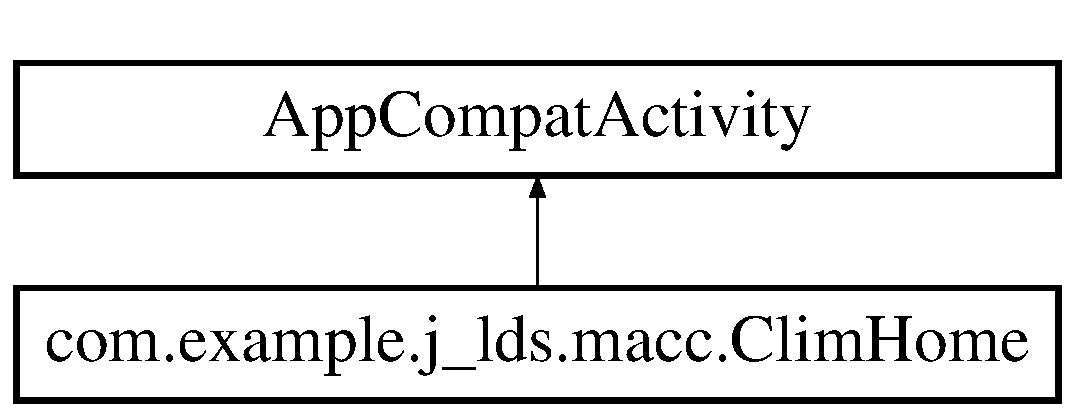
\includegraphics[height=2.000000cm]{a00024}
\end{center}
\end{figure}
\subsection*{Fonctions membres protégées}
\begin{DoxyCompactItemize}
\item 
\mbox{\Hypertarget{a00024_a5291ba568133ddc3781d5a5c00423103}\label{a00024_a5291ba568133ddc3781d5a5c00423103}} 
void {\bfseries on\+Create} (Bundle saved\+Instance\+State)
\item 
\mbox{\Hypertarget{a00024_a791abf995e0bfbe042b5d232bfa325b4}\label{a00024_a791abf995e0bfbe042b5d232bfa325b4}} 
void {\bfseries e4\+Csg1\+Macc\+\_\+on\+\_\+\+Off} ()
\item 
\mbox{\Hypertarget{a00024_ac4fe647dbee99df38770804e858146dc}\label{a00024_ac4fe647dbee99df38770804e858146dc}} 
void {\bfseries e4\+Csg1\+Macc\+\_\+plus} ()
\item 
\mbox{\Hypertarget{a00024_add576228d3eea662639b16bf2af54c93}\label{a00024_add576228d3eea662639b16bf2af54c93}} 
void {\bfseries e4\+Csg1\+Macc\+\_\+minus} ()
\item 
\mbox{\Hypertarget{a00024_a85d446f4cf76006b86fadeeeabb43687}\label{a00024_a85d446f4cf76006b86fadeeeabb43687}} 
String {\bfseries e4\+Csg1\+Macc\+\_\+mode} ()
\item 
\mbox{\Hypertarget{a00024_a537420aa4584bf16fc192ecdb07b0769}\label{a00024_a537420aa4584bf16fc192ecdb07b0769}} 
void {\bfseries e4\+Csg1\+Macc\+\_\+temp\+Graph} ()
\item 
\mbox{\Hypertarget{a00024_aa3393761ce82cd4ffcd83ba3d17690aa}\label{a00024_aa3393761ce82cd4ffcd83ba3d17690aa}} 
void {\bfseries e4\+Csg1\+Macc\+\_\+back\+Login} ()
\end{DoxyCompactItemize}


La documentation de cette classe a été générée à partir du fichier suivant \+:\begin{DoxyCompactItemize}
\item 
Clim\+Home.\+java\end{DoxyCompactItemize}

\hypertarget{a00036}{}\section{Référence de la classe com.\+example.\+j\+\_\+lds.\+macc.\+Connection\+Class}
\label{a00036}\index{com.\+example.\+j\+\_\+lds.\+macc.\+Connection\+Class@{com.\+example.\+j\+\_\+lds.\+macc.\+Connection\+Class}}
\subsection*{Fonctions membres publiques}
\begin{DoxyCompactItemize}
\item 
\mbox{\Hypertarget{a00036_a8062c1d9a0755d76fe2eab4abf78bcd9}\label{a00036_a8062c1d9a0755d76fe2eab4abf78bcd9}} 
Connection {\bfseries e4\+Csg1\+M\+A\+C\+C\+\_\+\+C\+O\+NN} ()
\end{DoxyCompactItemize}


La documentation de cette classe a été générée à partir du fichier suivant \+:\begin{DoxyCompactItemize}
\item 
Connection\+Class.\+java\end{DoxyCompactItemize}

\hypertarget{a00040}{}\section{Référence de la classe com.\+example.\+j\+\_\+lds.\+macc.\+find\+Salle\+Clim}
\label{a00040}\index{com.\+example.\+j\+\_\+lds.\+macc.\+find\+Salle\+Clim@{com.\+example.\+j\+\_\+lds.\+macc.\+find\+Salle\+Clim}}
Graphe d\textquotesingle{}héritage de com.\+example.\+j\+\_\+lds.\+macc.\+find\+Salle\+Clim\+:\begin{figure}[H]
\begin{center}
\leavevmode
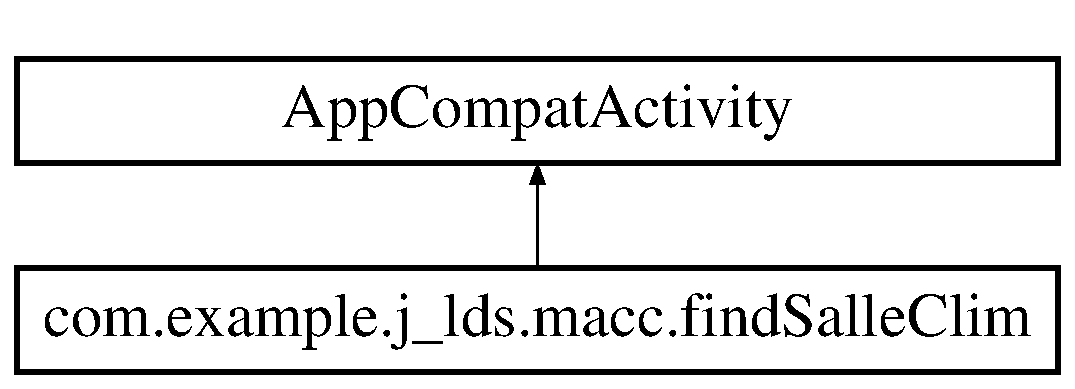
\includegraphics[height=2.000000cm]{a00040}
\end{center}
\end{figure}
\subsection*{Fonctions membres protégées}
\begin{DoxyCompactItemize}
\item 
\mbox{\Hypertarget{a00040_a259426547026c522e5a5c6b871ac49db}\label{a00040_a259426547026c522e5a5c6b871ac49db}} 
void {\bfseries on\+Create} (Bundle saved\+Instance\+State)
\end{DoxyCompactItemize}


La documentation de cette classe a été générée à partir du fichier suivant \+:\begin{DoxyCompactItemize}
\item 
find\+Salle\+Clim.\+java\end{DoxyCompactItemize}

\hypertarget{a00044}{}\section{Référence de la classe com.\+example.\+j\+\_\+lds.\+macc.\+Login\+Home}
\label{a00044}\index{com.\+example.\+j\+\_\+lds.\+macc.\+Login\+Home@{com.\+example.\+j\+\_\+lds.\+macc.\+Login\+Home}}
Graphe d\textquotesingle{}héritage de com.\+example.\+j\+\_\+lds.\+macc.\+Login\+Home\+:\begin{figure}[H]
\begin{center}
\leavevmode
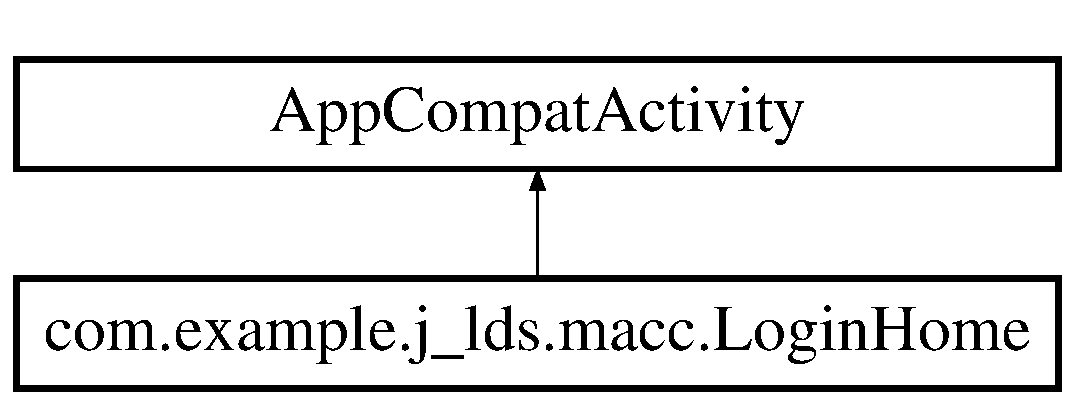
\includegraphics[height=2.000000cm]{a00044}
\end{center}
\end{figure}
\subsection*{Fonctions membres protégées}
\begin{DoxyCompactItemize}
\item 
\mbox{\Hypertarget{a00044_ae5a72dc4fded6a8c56a7268952a372ec}\label{a00044_ae5a72dc4fded6a8c56a7268952a372ec}} 
void {\bfseries on\+Create} (Bundle saved\+Instance\+State)
\end{DoxyCompactItemize}


La documentation de cette classe a été générée à partir du fichier suivant \+:\begin{DoxyCompactItemize}
\item 
Login\+Home.\+java\end{DoxyCompactItemize}

\hypertarget{a00052}{}\section{Référence de la classe com.\+example.\+j\+\_\+lds.\+macc.\+Temperature\+Graph}
\label{a00052}\index{com.\+example.\+j\+\_\+lds.\+macc.\+Temperature\+Graph@{com.\+example.\+j\+\_\+lds.\+macc.\+Temperature\+Graph}}
Graphe d\textquotesingle{}héritage de com.\+example.\+j\+\_\+lds.\+macc.\+Temperature\+Graph\+:\begin{figure}[H]
\begin{center}
\leavevmode
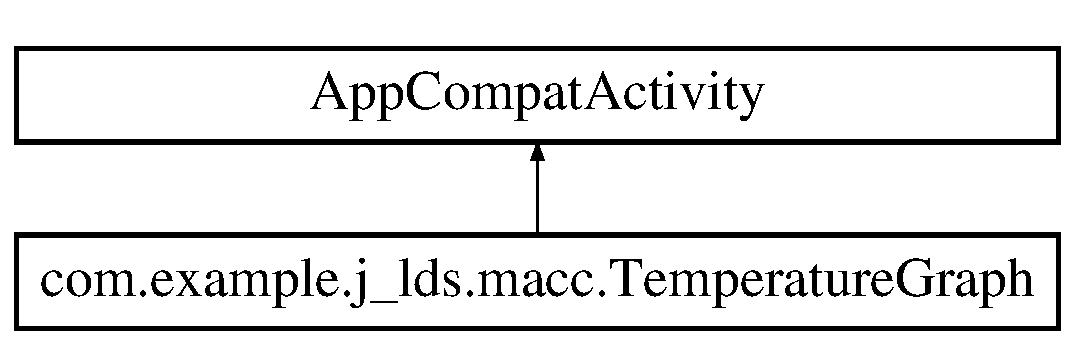
\includegraphics[height=2.000000cm]{a00052}
\end{center}
\end{figure}
\subsection*{Classes}
\begin{DoxyCompactItemize}
\item 
class {\bfseries e4\+Csg1\+M\+A\+C\+C\+\_\+my\+Task}
\end{DoxyCompactItemize}
\subsection*{Fonctions membres publiques}
\begin{DoxyCompactItemize}
\item 
\mbox{\Hypertarget{a00052_aecd489a18fb620f05878526d1b903578}\label{a00052_aecd489a18fb620f05878526d1b903578}} 
Data\+Point \mbox{[}$\,$\mbox{]} {\bfseries get\+Data\+Point} ()
\item 
\mbox{\Hypertarget{a00052_a82f17820dd387201db287d74bf1968b7}\label{a00052_a82f17820dd387201db287d74bf1968b7}} 
void {\bfseries back\+Home} ()
\end{DoxyCompactItemize}
\subsection*{Fonctions membres protégées}
\begin{DoxyCompactItemize}
\item 
\mbox{\Hypertarget{a00052_a725657d4ff9d5c93aad83343b01f304d}\label{a00052_a725657d4ff9d5c93aad83343b01f304d}} 
void {\bfseries on\+Create} (Bundle saved\+Instance\+State)
\end{DoxyCompactItemize}


La documentation de cette classe a été générée à partir du fichier suivant \+:\begin{DoxyCompactItemize}
\item 
Temperature\+Graph.\+java\end{DoxyCompactItemize}

%--- End generated contents ---

% Index
\backmatter
\newpage
\phantomsection
\clearemptydoublepage
\addcontentsline{toc}{chapter}{Index}
\printindex

\end{document}
